\section{Experiments}\label{sec:experiments}

\subsection{Plan}

Experiment setup

\begin{itemize}
    \item Scanner memory size (currently 32 GB), can go down to 5 GB
    \item Scanner number of CPU cores
    \item Sample size (current 1M, 5M)
    \item How much it costs $TrainingTime \times NumOfScanners \times CostPerHour$
    \item size of trees (1 stump, 3=1root+2stumps, 7=1root+2trees)
    \item random vs non-random tree root
    \item splice and bathymetry dataset
    \item number of machines, 1, 10, 100
    \item run for 6000 seconds
\end{itemize}

Evaluation

\begin{itemize}
    \item Number of examples scanned per unit time (average over all scanners)
    
\end{itemize}

\subsection{Content}

In this section we describe the results of experiments comparing
the run time of \Sparrow\ with those of two leading implementations of
boosted trees: XGBoost and LightGBM.


\begin{table}[]
\centering
\begin{tabular}{|r|r|r|r|}
\hline
Memory       & \Sparrow         & XGBoost             & LightGBM       \\ \hline
16 GB        & 18.5 (d)         & 3224.7 (d) & (crash)        \\
32 GB        & 17.9 (d)         & 1705.8 (d) & (crash)        \\
72 GB        & 21.9 (d)         & 1497.7 (d) & 108.1 (m)          \\
144 GB       & 19.6 (d)         & 241.4  (m) & 109.4 (m)         \\ \hline

% \end{tabular}
% \vspace{0.2cm}
% \begin{tabular}{|l|l|c|c|}
%                 & \Sparrow         & XGBoost             & LightGBM       \\ \hline
\#~Rules  & 189    & 400                 & 400            \\ \hline
\end{tabular}

\vspace{0.2cm}

\caption{Comparison of the total training time on
the splice site detection task (minutes) and the number
of rules in the final ensemble when it converges.
The (m) suffix denotes the package loads all training data to memory.
The (d) suffix denotes the package does not load all training data to memory and uses disk
as the external memory.
}\label{table-exp}
\end{table}

\begin{table}[]
\centering
\begin{tabular}{|r|r|r|r|}
\hline
Memory       & \Sparrow            & XGBoost    & LightGBM       \\ \hline
16 GB        & 5.7 (d)             & 483.7 (d)  & (crash)        \\
32 GB        & 5.6 (d)             & 255.9 (d)  & (crash)        \\
72 GB        & 6.8 (d)             & 224.7 (d)  & 16.2 (d)          \\
144 GB       & 6.6 (d)             & 36.2 (m)   & 16.4 (d)          \\ \hline
\end{tabular}

\vspace{0.2cm}

\caption{Comparison of the per-tree training time
on the splice site detection task (seconds).
The (m) suffix denotes the package loads all training data to memory.
The (d) suffix denotes the package does not load all training data to memory and uses disk
as the external memory.}\label{table-per-tree}
\end{table}


\subsection{Setup}

We use a large dataset that was used in other studies of large scale
learning on detecting human acceptor splice site~\cite{sonnenburg_coffin_2010, agarwal_reliable_2014}.
The learning task is binary classification.
We use the same training dataset of 50\,M samples as in the other work,
and validate the model on the testing data set of 4.6\,M samples.
The training dataset on disk takes over 27\,GB in size.

In current implementation of \Sparrow, we restrict our trees to one
level so-called ``decision stumps''. We plan to perform comparisons
using multi-level trees and more than two labels. We expect similar
runtime performance there. To generate comparable models,
we also train decision stumps in XGBoost and LightGBM
(by setting the maximum tree depth to 1).

Both XGBoost and LightGBM are highly optimized, and support multiple
tree construction algorithms.
For XGBoost, we chose approximate greedy algorithm which is its fastest method.
LightGBM supports using sampling in the training,
which they called \textit{Gradient-based One-Side Sampling} (GOSS).
GOSS keeps a fixed percentage of examples with large gradients,
and then randomly sample from remaining examples with small gradients.
We selected GOSS as the tree construction algorithm for LightGBM.

All algorithms in comparison optimize the exponential loss as defined in AdaBoost.
We also evaluated the final model by calculating its area under precision-recall
curve (AUPRC) on the testing dataset.

Finally, the experiments are all conducted on EC2 instances from Amazon Web Services.
We ran the evaluations on four different instance types with increasing memory capacities,
specifically
16\,GB (\texttt{c5d.2xlarge}), 32\,GB (\texttt{c5d.2xlarge}),
72\,GB (\texttt{c5d.9xlarge}), and 144\,GB (\texttt{c5d.18xlarge}).
The memory requirement of \Sparrow\ is decided by the sample size,
which is a configurable parameter.
XGBoost supports external memory training when the memory is too small to fit the
training dataset.
Unlike XGBoost, LightGBM does not support external memory execution.


\subsection{Evaluation}

We compare \Sparrow\ XGBoost and LightGBM. The comparison was done in
terms of the reduction in the exponential loss which is what boosting
minimizes directly and in terms of a AUPRC which is often more
relevant for practice.

Performance of each of the algorithm in terms of
the exponential loss as a function of time on the testing dataset is given in
Figure~\ref{fig:loss}. Observe that all algorithms achieve similar
final loss, but it takes them different amount of time to reach that
final loss.
In the most limited memory setting (16 GB),
XGBoost external memory is about 174x
 slower than \Sparrow\ which also uses external memory.
Even comparing to the in-memory versions of LightGBM and XGBoost,
\Sparrow\ is 6x and 13x faster, respectively.

In Figure~\ref{fig:auprc} we perform the comparison in terms of
AUPRC. The results are similar in terms of speed. However, in this
case XGBoost and LightGBM ultimately achieve a slightly better
AUPRC. This is baffling, because all algorithms work by minimizing
exponential loss.

We summarize the experiments results in Table~\ref{table-exp} by
using the convergence time to an almost optimal exponential loss of $0.061$.
Table~\ref{table-per-tree} lists the per-tree training time of each packages
in different memory settings.
The in-memory version of XGBoost runs out of memory on the instances with
the memory sizes of 16-72 GB. We trained the model using the external memory
version on those instances.

\begin{figure}[t]
    \centering
    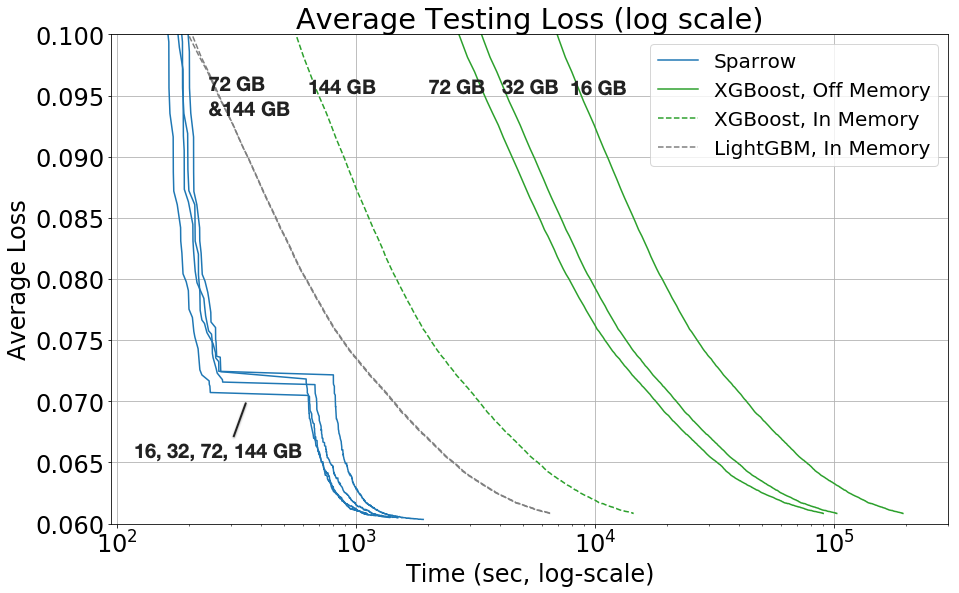
\includegraphics[width=0.5\textwidth]{figs/splice-loss2m.png}
    \caption{Comparing the average loss on the testing data using \Sparrow, XGBoost, and LightGBM, lower is better.
        The period of time that the loss is constant for \Sparrow\ is when the algorithm is generating a new sample set.}~\label{fig:loss}
\end{figure}

\begin{figure}[t]
    \centering
    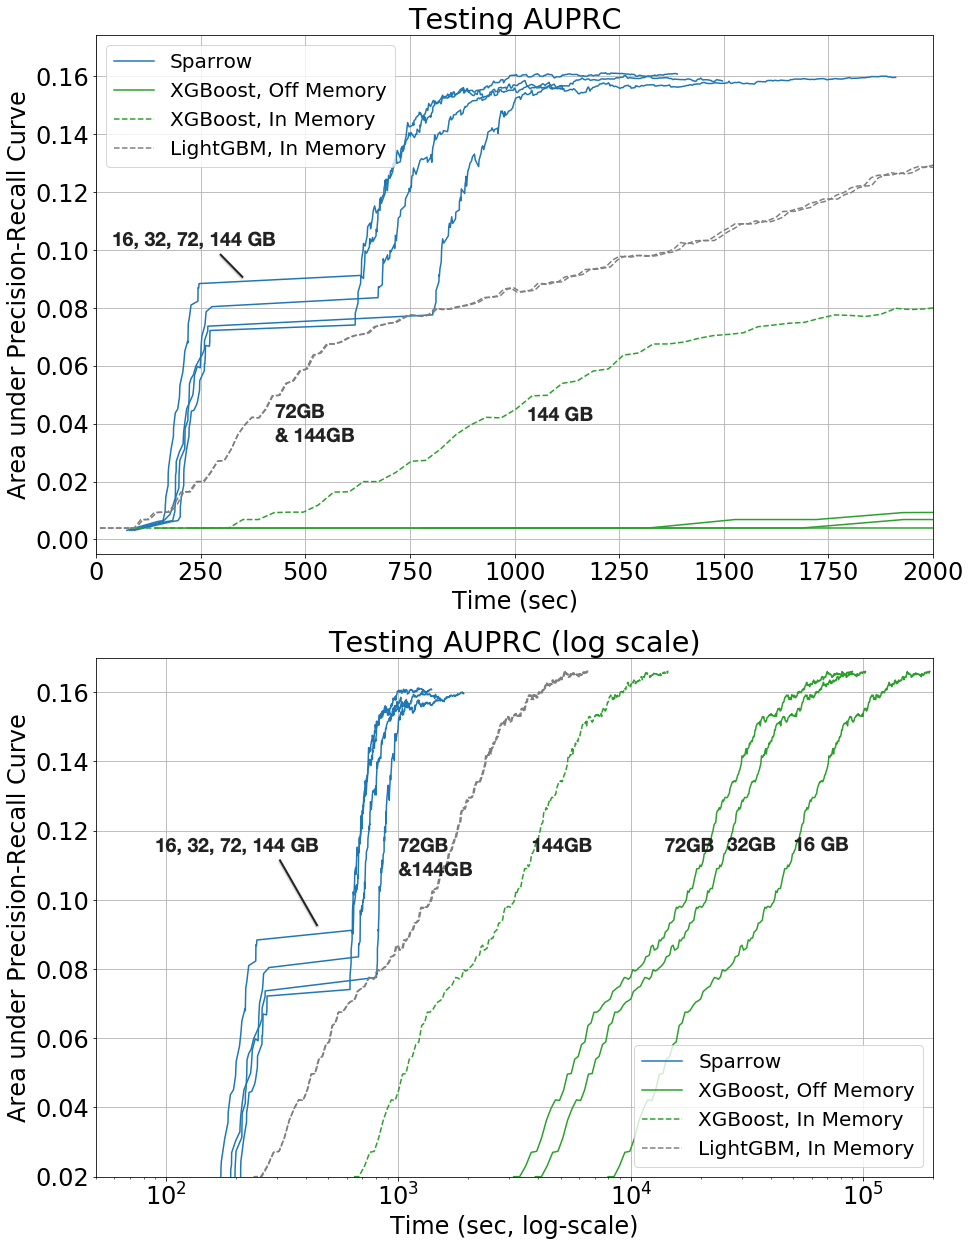
\includegraphics[width=0.5\textwidth]{figs/splice-auprc2m.png}
    \caption{Comparing the area under the precision-recall curve (AUPRC) on the testing data
    using \Sparrow, XGBoost, and LightGBM, higher is better.
    (left) Normal scale, clipped on right.
    (right) Log scale, clipped on left.
    The period of time that the AUPRC is constant for \Sparrow\ is when the algorithm is generating a new sample set.}~\label{fig:auprc}
\end{figure}


\section{Future Work}\label{sec:Conclusion}
Our preliminary results show that early stopping and selective
sampling can dramatically speed up boosting algorithms on large
real-world datasets.

The source code for \Sparrow\ will be released with the
final version of the paper.

We have several directions for future work.

First, \Sparrow\ is currently limited boosting stumps and to binary
classification. We plan to extend \Sparrow\ to deep trees and to allow
more than two labels. We will then run it on many more data sets.

Second, our work shows that sampling from memory can take an
inordinate amount of time when the training set is large and the
weights are highly skewed. We have developed a stratified sampling
algorithm that significantly reduces this problem.

Third, we are working on a parallelized version of \Sparrow\ which
uses a  novel type of asynchronous communication protocol.

Fourth, our current implementation of \Sparrow\ does not take
advantage of multi-core machines as much as LightGBM does. We plan to
address that problem.




